\tikzstyle{input_neuron}=[circle,draw=red!50,fill=orange!10,thick,minimum size=6mm]
\tikzstyle{hidden_neuron}=[circle,draw=blue!50,fill=blue!10,thick,minimum size=6mm]
\tikzstyle{output_neuron}=[circle,draw=green!50,fill=green!20,thick,minimum size=6mm]
\tikzstyle{input}=[circle,draw=black!50,fill=black!20,thick,minimum size=6mm]

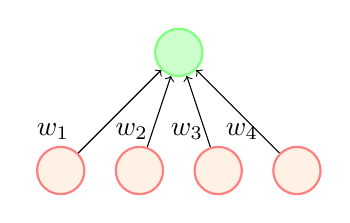
\begin{tikzpicture}

	\node [output_neuron] (out_neuron0) at (2.5,4){};
	\node [input_neuron] (input_neuron1) at (1,2.5){};
	\node [input_neuron] (input_neuron2) at (2,2.5){};
	\node [input_neuron] (input_neuron3) at (3,2.5){};
	\node [input_neuron] (input_neuron4) at (4,2.5){};
	\draw [->] (input_neuron1) -- (out_neuron0);
	\draw [->] (input_neuron2) -- (out_neuron0);
	\draw [->] (input_neuron3) -- (out_neuron0);
	\draw [->] (input_neuron4) -- (out_neuron0);
	\node[text width=0.005cm] at (0.7,3) {$w_1$};
	\node[text width=0.005cm] at (1.7,3) {$w_2$};
	\node[text width=0.005cm] at (2.4,3) {$w_3$};
	\node[text width=0.005cm] at (3.1,3) {$w_4$};
	
\end{tikzpicture}